\documentclass{article}
\PassOptionsToPackage{table}{xcolor}
\usepackage{geometry}
\usepackage{tikz}
\usepackage[most]{tcolorbox}
\usepackage{mathabx}
\usepackage{booktabs}
\usepackage{tabularx}
\usepackage{nicefrac}
\usepackage{pdflscape}

\usetikzlibrary{tikzmark}

% https://tex.stackexchange.com/questions/198658/
\makeatletter
\newcommand\incircbin
{\mathpalette\@incircbin}
\newcommand\@incircbin[2]
{\mathbin{\ooalign{\hidewidth$#1#2$\hidewidth\crcr$#1\ovoid$}}}
\newcommand{\ocol}{\incircbin{\raisebox{0.4pt}{:}}}
\newcommand{\shrinkstack}[1]{\tikzmarknode[fill=instr-shrink-stack,circle,inner sep=-1pt]{circ}{#1}}
\makeatother

\geometry{a4paper, total={170mm, 257mm}, left=20mm}
\linespread{1.9}

\tcbset{on line, box align=base,
    sharp corners=northwest,sharp corners=southeast,
    boxsep=4pt, left=0pt,right=0pt,top=0pt,bottom=0pt,
    grow to left by=5pt,
    colframe=white
}
\newcommand{\splitbox}[3]{
    \tcbox[enhanced, interior code={%
        \path[fill=#1,rounded corners=5px] (interior.north west) |- (interior.south east);
        \path[fill=#2,rounded corners=5px] (interior.south east) |- (interior.north west);
    }]{#3}
}

\colorlet{instr-arg}{red!30!green!20}
\colorlet{instr-jsp}{blue!90!green!20}
\colorlet{instr-shrink-stack}{yellow!50}
\colorlet{hint}{gray}
\colorlet{row1}{white}
\colorlet{row2}{gray!8}

% declared as commands purely for reasons of latex source code formatting
\newcommand{\hintdivinesib}{
    \textcolor{hint}{\texttt{st12 \% 2 = 0 $\Rightarrow$ left node}}
}
\newcommand{\hintsplit}{
    \textcolor{hint}{\texttt{hi $\rightarrow$ st0'}}
}
\newcommand{\hintlt}{
    \textcolor{hint}{\texttt{st0} $\stackrel{\texttt{?}}{\texttt{<}}$ \texttt{st1}}
}
\newcommand{\hintdiv}{
    \textcolor{hint}{\nicefrac{\texttt{st0}}{\texttt{st1}}}
}
\newcommand{\hintxbmul}{
    \textcolor{hint}{\texttt{st0 $\cdot$ (st1, st2, st3)}}
}

\newcommand{\ssominus}{
    \shrinkstack{\ensuremath{\ominus}}
}

\begin{document}
\pagestyle{empty}
\begin{minipage}{0.3\textwidth}
\begin{tabular}{rlll}
    \texttt{02} & $\ssominus$   & \texttt{pop}                                       &                \\
    \texttt{01} & $\oplus$      & \tcbox[colback=instr-arg]{\texttt{push + a}}       &                \\
    \texttt{04} & $\oplus$      & \texttt{divine}                                    &                \\
    \texttt{05} & $\oplus$      & \tcbox[colback=instr-arg]{\texttt{dup + i}}        &                \\
    \texttt{09} & $\ovoid^{16}$ & \tcbox[colback=instr-arg]{\texttt{swap + i}}       &                \\
    \texttt{08} & $\ovoid$      & \texttt{nop}                                       &                \\
    \texttt{06} & $\ssominus$   & \tcbox[colback=instr-jsp]{\texttt{skiz}}           &                \\
    \texttt{13} & $\ovoid$      & \splitbox{instr-jsp}{instr-arg}{\texttt{call + d}} &                \\
    \texttt{12} & $\ovoid$      & \tcbox[colback=instr-jsp]{\texttt{return}}         &                \\
    \texttt{16} & $\ovoid$      & \tcbox[colback=instr-jsp]{\texttt{recurse}}        &                \\
    \texttt{10} & $\ssominus$   & \texttt{assert}                                    &                \\
    \texttt{00} & $\ovoid$      & \texttt{halt}                                      &                \\
    \texttt{20} & $\ovoid^1$    & \texttt{read\_mem}                                 &                \\
    \texttt{24} & $\ovoid$      & \texttt{write\_mem}                                &                \\
    \texttt{28} & $\ovoid^{10}$ & \texttt{hash}                                      &                \\
    \texttt{32} & $\ovoid^{11}$ & \texttt{divine\_sibling}                           & \hintdivinesib \\
    \texttt{36} & $\ovoid$      & \texttt{assert\_vector}                            &                \\
    \texttt{14} & $\ssominus^1$ & \texttt{add}                                       &                \\
    \texttt{18} & $\ssominus^1$ & \texttt{mul}                                       &                \\
    \texttt{40} & $\ovoid^1$    & \texttt{invert}                                    &                \\
    \texttt{44} & $\oplus^2$    & \texttt{split}                                     & \hintsplit     \\
    \texttt{22} & $\ssominus^1$ & \texttt{eq}                                        &                \\
    \texttt{48} & $\oplus^2$    & \texttt{lsb}                                       &                \\
    \texttt{52} & $\ovoid^3$    & \texttt{xxadd}                                     &                \\
    \texttt{56} & $\ovoid^3$    & \texttt{xxmul}                                     &                \\
    \texttt{60} & $\ovoid^3$    & \texttt{xinvert}                                   &                \\
    \texttt{26} & $\ssominus^3$ & \texttt{xbmul}                                     & \hintxbmul     \\
    \texttt{64} & $\oplus$      & \texttt{read\_io}                                  &                \\
    \texttt{30} & $\ssominus$   & \texttt{write\_io}                                 &
\end{tabular}
\end{minipage}\hfill%
\begin{minipage}[][0.84\textheight][s]{0.6\textwidth}
    \rowcolors{3}{row1}{row2}
    \hfill
    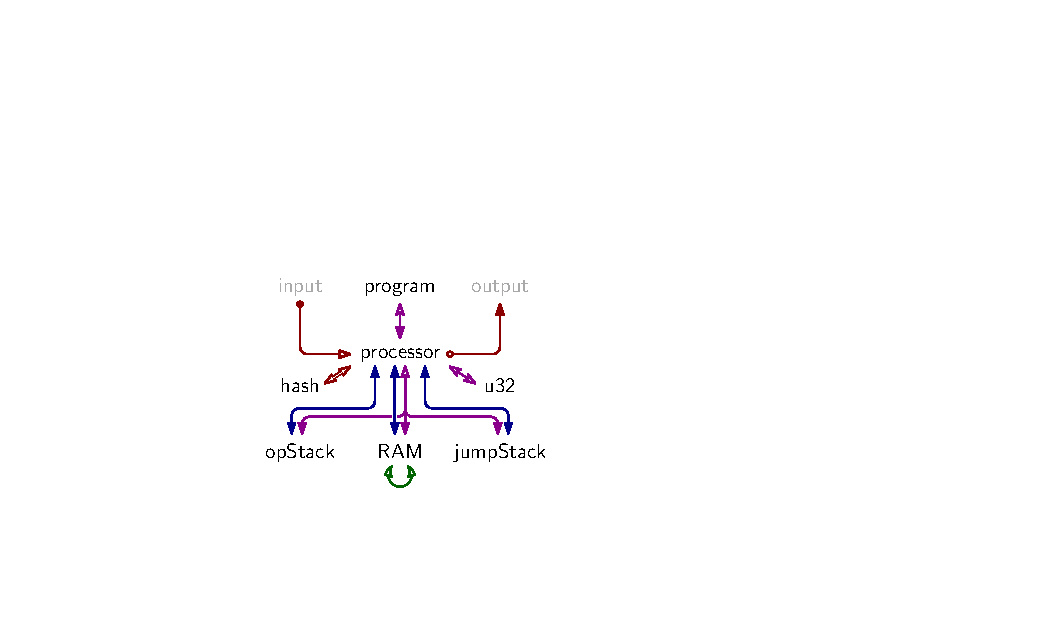
\includegraphics[keepaspectratio,width=0.9\textwidth]{src/img/aet-relations.pdf}
    \vfill

    \hfill
    \begin{tabular}{lrr}
        \multicolumn{3}{l}{\small $p = 18446744069414584321$} \\ \toprule
        $i$ & $\nicefrac{1}{i}$ &          $\nicefrac{-1}{i}$ \\ \midrule
        2   &     092\dots\!161 &               922\dots\!160 \\
        3   &     122\dots\!881 &               614\dots\!440 \\
        4   &     138\dots\!241 &               461\dots\!080 \\
        5   &     147\dots\!457 &               368\dots\!864 \\
        6   &     153\dots\!601 &               307\dots\!720 \\ \bottomrule
    \end{tabular}
    \vfill

    \hfill
    \rowcolors{2}{row2}{row1}
    \begin{tabular}{lrrr}
        \toprule
                    & base & ext & $\sum$ \\ \midrule
        Program     &    3 &   1 &      4 \\
        Instruction &    4 &   2 &      6 \\
        Processor   &   42 &  11 &     53 \\
        OpStack     &    5 &   2 &      7 \\
        RAM         &    7 &   6 &     13 \\
        JumpStack   &    6 &   2 &      8 \\
        Hash        &   49 &   2 &     51 \\ \bottomrule\bottomrule
        $\sum$      &  116 &  26 &    142
    \end{tabular}
\end{minipage}

\newpage
\hspace*{-4em}%
\scalebox{0.75}{
    \rowcolors{2}{row2}{row1}
\begin{tabular}{lllllllllllllllllllllll}
    \toprule
    Table       & \multicolumn{5}{l}{Base Columns}                                                &              &                     &              &              &              &              &              &       &               &              &              &              &       &              &               &               &               \\ \midrule
    Program     & \multicolumn{3}{l}{Address}                   & \multicolumn{2}{l}{Instruction} & \multicolumn{3}{l}{IsPadding}                     &              &              &              &              &       &               &              &              &              &       &              &               &               &               \\
    Instruction & \multicolumn{3}{l}{Address}                   & \texttt{CI} & \texttt{NIA}      & \multicolumn{3}{l}{IsPadding}                     &              &              &              &              &       &               &              &              &              &       &              &               &               &               \\
    Processor   & \texttt{CLK} & IsPadding        & \texttt{IP} & \texttt{CI} & \texttt{NIA}      & \texttt{IB0} & \dots               & \texttt{IB6} & \texttt{JSP} & \texttt{JSO} & \texttt{JSD} & \texttt{ST0} & \dots & \texttt{ST15} & \texttt{OSP} & \texttt{OSV} & \texttt{HV0} & \dots & \texttt{HV3} & \texttt{RAMP} & \texttt{RAMV} &               \\
    OpStack     & \texttt{CLK} & \texttt{clk\_di} &             &             &                   &              & \multicolumn{4}{l}{\texttt{IB1} ($\widehat{=}$ shrink stack)}    &              &              &       &               & \texttt{OSP} & \texttt{OSV} &              &       &              &               &               &               \\
    RAM         & \texttt{CLK} & \texttt{clk\_di} &             &             & \texttt{bcpc0}    & \multicolumn{2}{l}{\texttt{bcpc1}} &              &              &              &              &              &       &               &              &              &              &       &              & \texttt{RAMP} & \texttt{RAMV} & \texttt{IORD} \\
    JumpStack   & \texttt{CLK} & \texttt{clk\_di} &             & \texttt{CI} &                   &              &                     &              & \texttt{JSP} & \texttt{JSO} & \texttt{JSD} &              &       &               &              &              &              &       &              &               &               &               \\
    Hash        & \multicolumn{4}{l}{RoundNumber}                             &                   &              &                     &              &              &              &              & \texttt{ST0} & \dots & \texttt{ST15} & \multicolumn{3}{l}{\texttt{CONSTANT0A}}    & \dots & \multicolumn{3}{l}{\texttt{CONSTANT15B}}     &               \\ \bottomrule
\end{tabular}
} %end scalebox
\vfill%
\begin{minipage}{0.3\textwidth}
    \rowcolors{2}{row2}{row1}
    \begin{tabular}{rl}
        \toprule
        \#clk & instruction            \\ \midrule
            2 & \texttt{neg}           \\
            4 & \texttt{sub}           \\
           68 & \texttt{is\_u32}       \\
          139 & \texttt{split\_assert} \\
          146 & \texttt{lte}           \\
          148 & \texttt{lt}            \\
          295 & \texttt{and}           \\
          301 & \texttt{xor}           \\
          195 & \texttt{reverse}       \\
          164 & \texttt{div}           \\ \bottomrule
    \end{tabular}
\end{minipage}

\end{document}
